\documentclass{article} % Oder eine andere Dokumentklasse wie report, book, etc.
\usepackage[utf8]{inputenc} % Bestimmt die Eingabe-Kodierung
\usepackage[T1]{fontenc} % Bestimmt die Ausgabe-Kodierung
\usepackage{graphicx}


\begin{document}
	
	\title{Deep Reinforcement Learning Exercise 01}
	\maketitle
	
	\section{Exercise 1.1}
	\subsection{1.1a}
	
	We implemented the epsilon-greedy algorithm with 2000 pulls out of a choice of 4 bandits. The pull probability is distributed as 0.1, 0.3, 0.5 and 0.7 for the four bandits (1-4). The results were averaged over 100 runs. 
	
	Figure \ref{fig:1.1.a.1} shows the results of the approach. The model explores in the beginning therefore accumulating more regret. As we can see, the epsilon-greedy algorithm is able to find the best bandit over time. However, at first it is not able to find the best bandit, as it explores other bandits and accumulates regret. After a certain number of pulls, it finds the best bandit and exploits it, resulting in more accumulated reward. 
	
	\begin{figure}[h!]
		\centering
		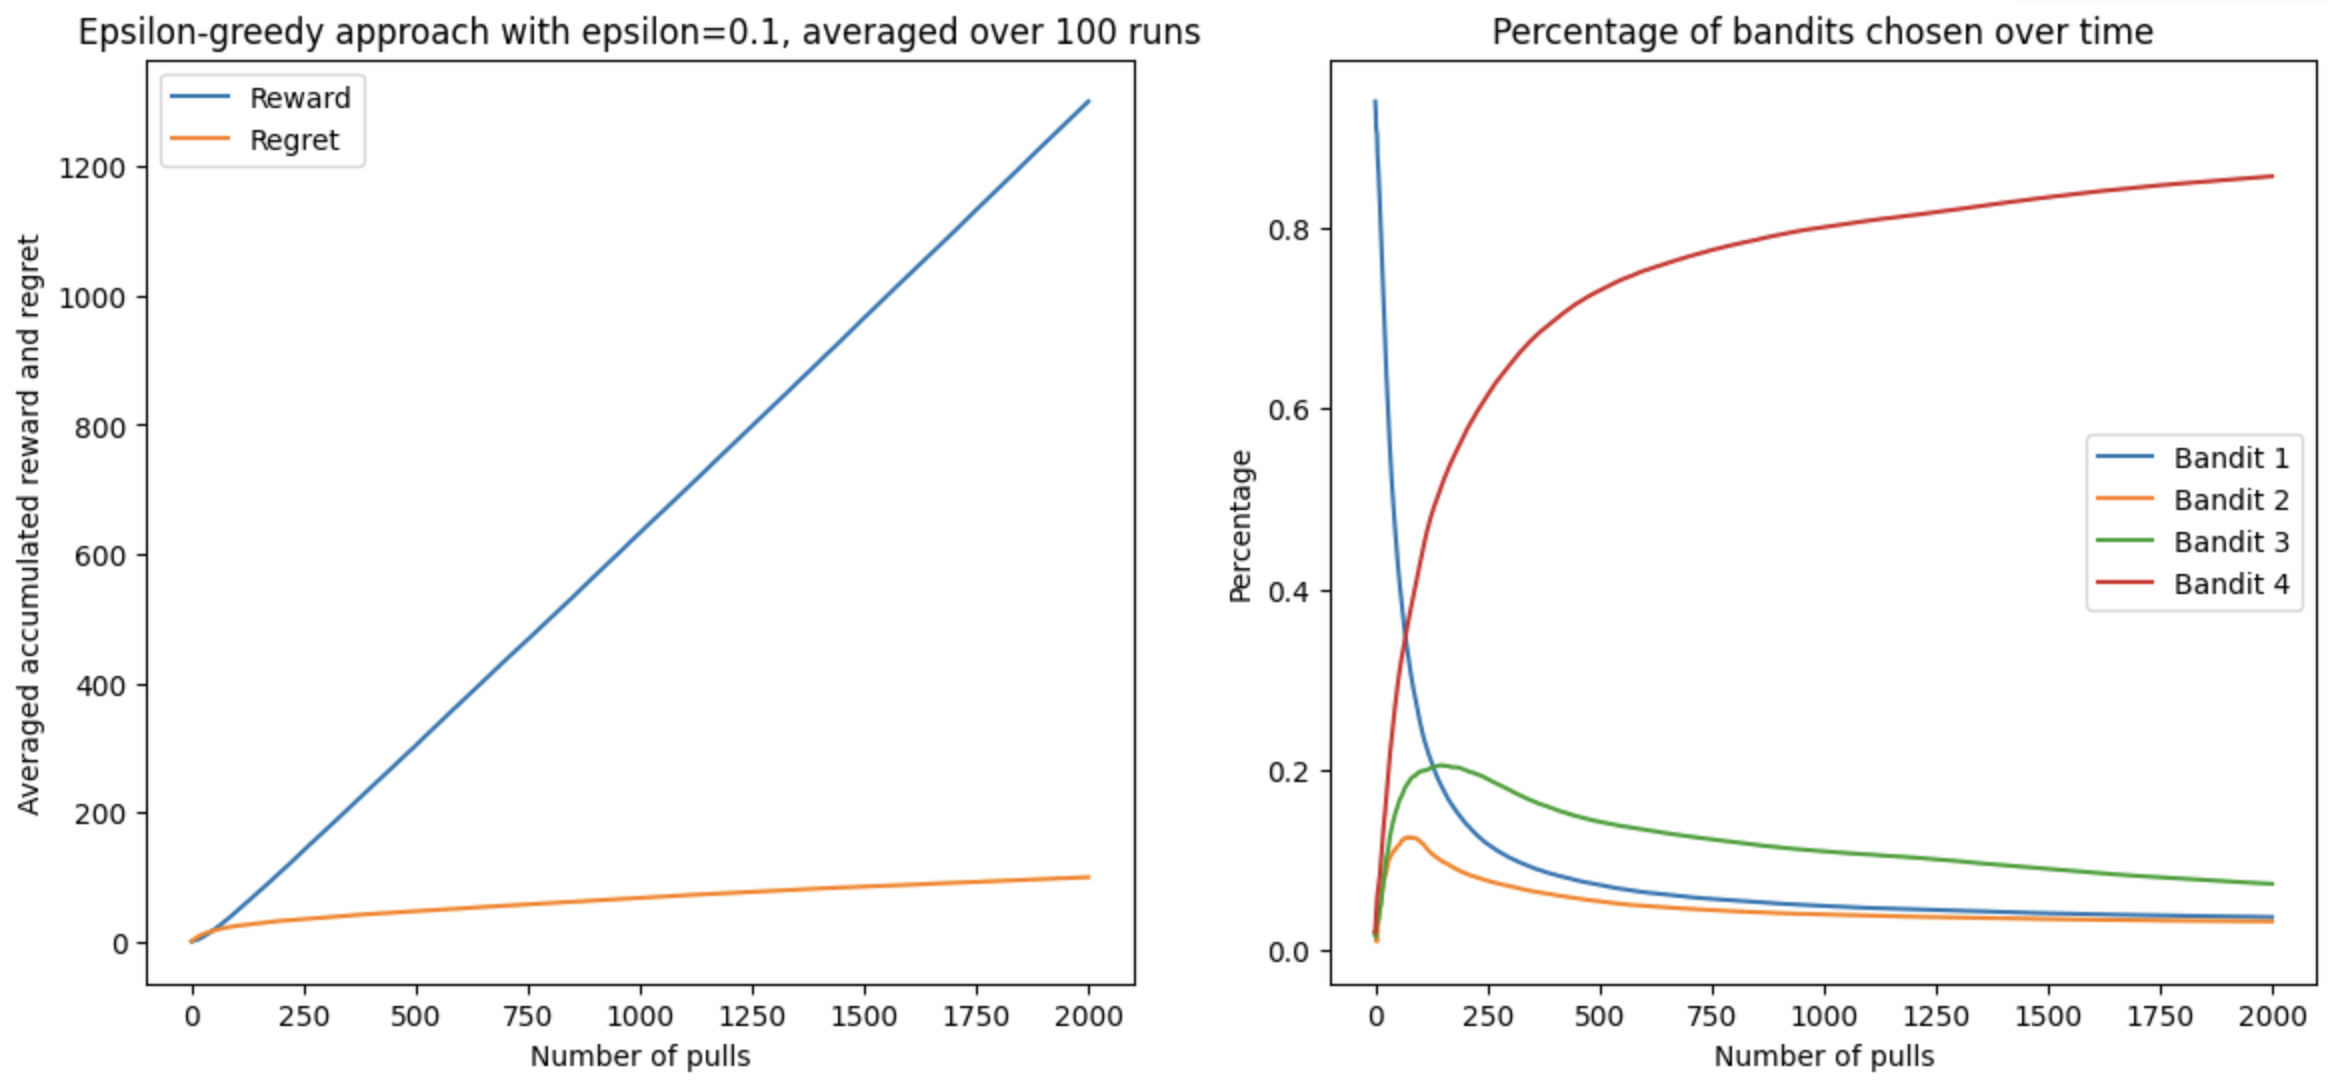
\includegraphics[width=0.9\textwidth]{images/1.1.a.1}
		\caption{Epsilon-greedy approach with epsilon = 0,1 averaged over 100 runs (left) and Percentage of bandits chosen over time (right)}
		\label{fig:1.1.a.1}
	\end{figure}
	
	This change over time is also represented in Figure \ref{fig:1.1.a.2}, where the estimated mean of each bandit over time is displayed. Bandit 4 has the highest actual mean reward, which the model quickly realizes and therefore uses it more often, which consequently leads to the rise of the estimated mean of Bandit 4. 
	
	\begin{figure}[h!]
		\centering
		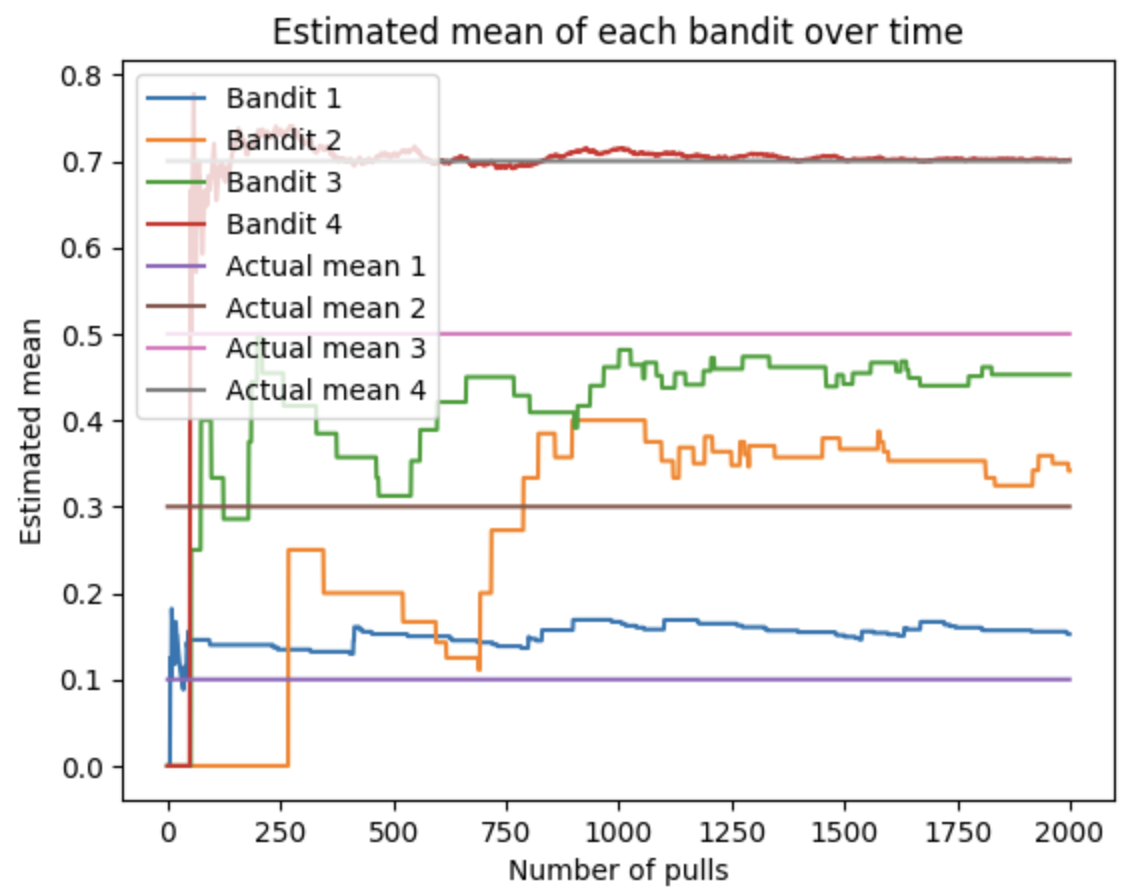
\includegraphics[width=0.8\textwidth]{images/1.1.a.2}
		\caption{Estimated mean of each bandit over time}
		\label{fig:1.1.a.2}
	\end{figure}

	\subsection{1.1b}
	
	Learnings: The higher the epsilon value, the more exploring happens in the beginning (with a factor of epsilon). The higher the epsilon, the fast the algorithm discovers the best bandit. But ultimately, the algorithm can only exploit it with a probability of 1-epsilon. 
	
	On the other hand, the lower the epsilon value, the longer it takes to to find the best bandit. This delay is then rewarded with better exploitation of the best bandit since less exploration takes place. 
	
	For these reasons, choosing a low epsilon will be advantageous in the long run. In our example (see \ref{fig:1.1.b}), the lowest epsilon however is barely outperforming the highest epsilon value while generating less reward than the middle epsilon value. But with more runs, the lowest epsilon value will outperform its competitors. 
	
	\begin{figure}[h!]
		\centering
		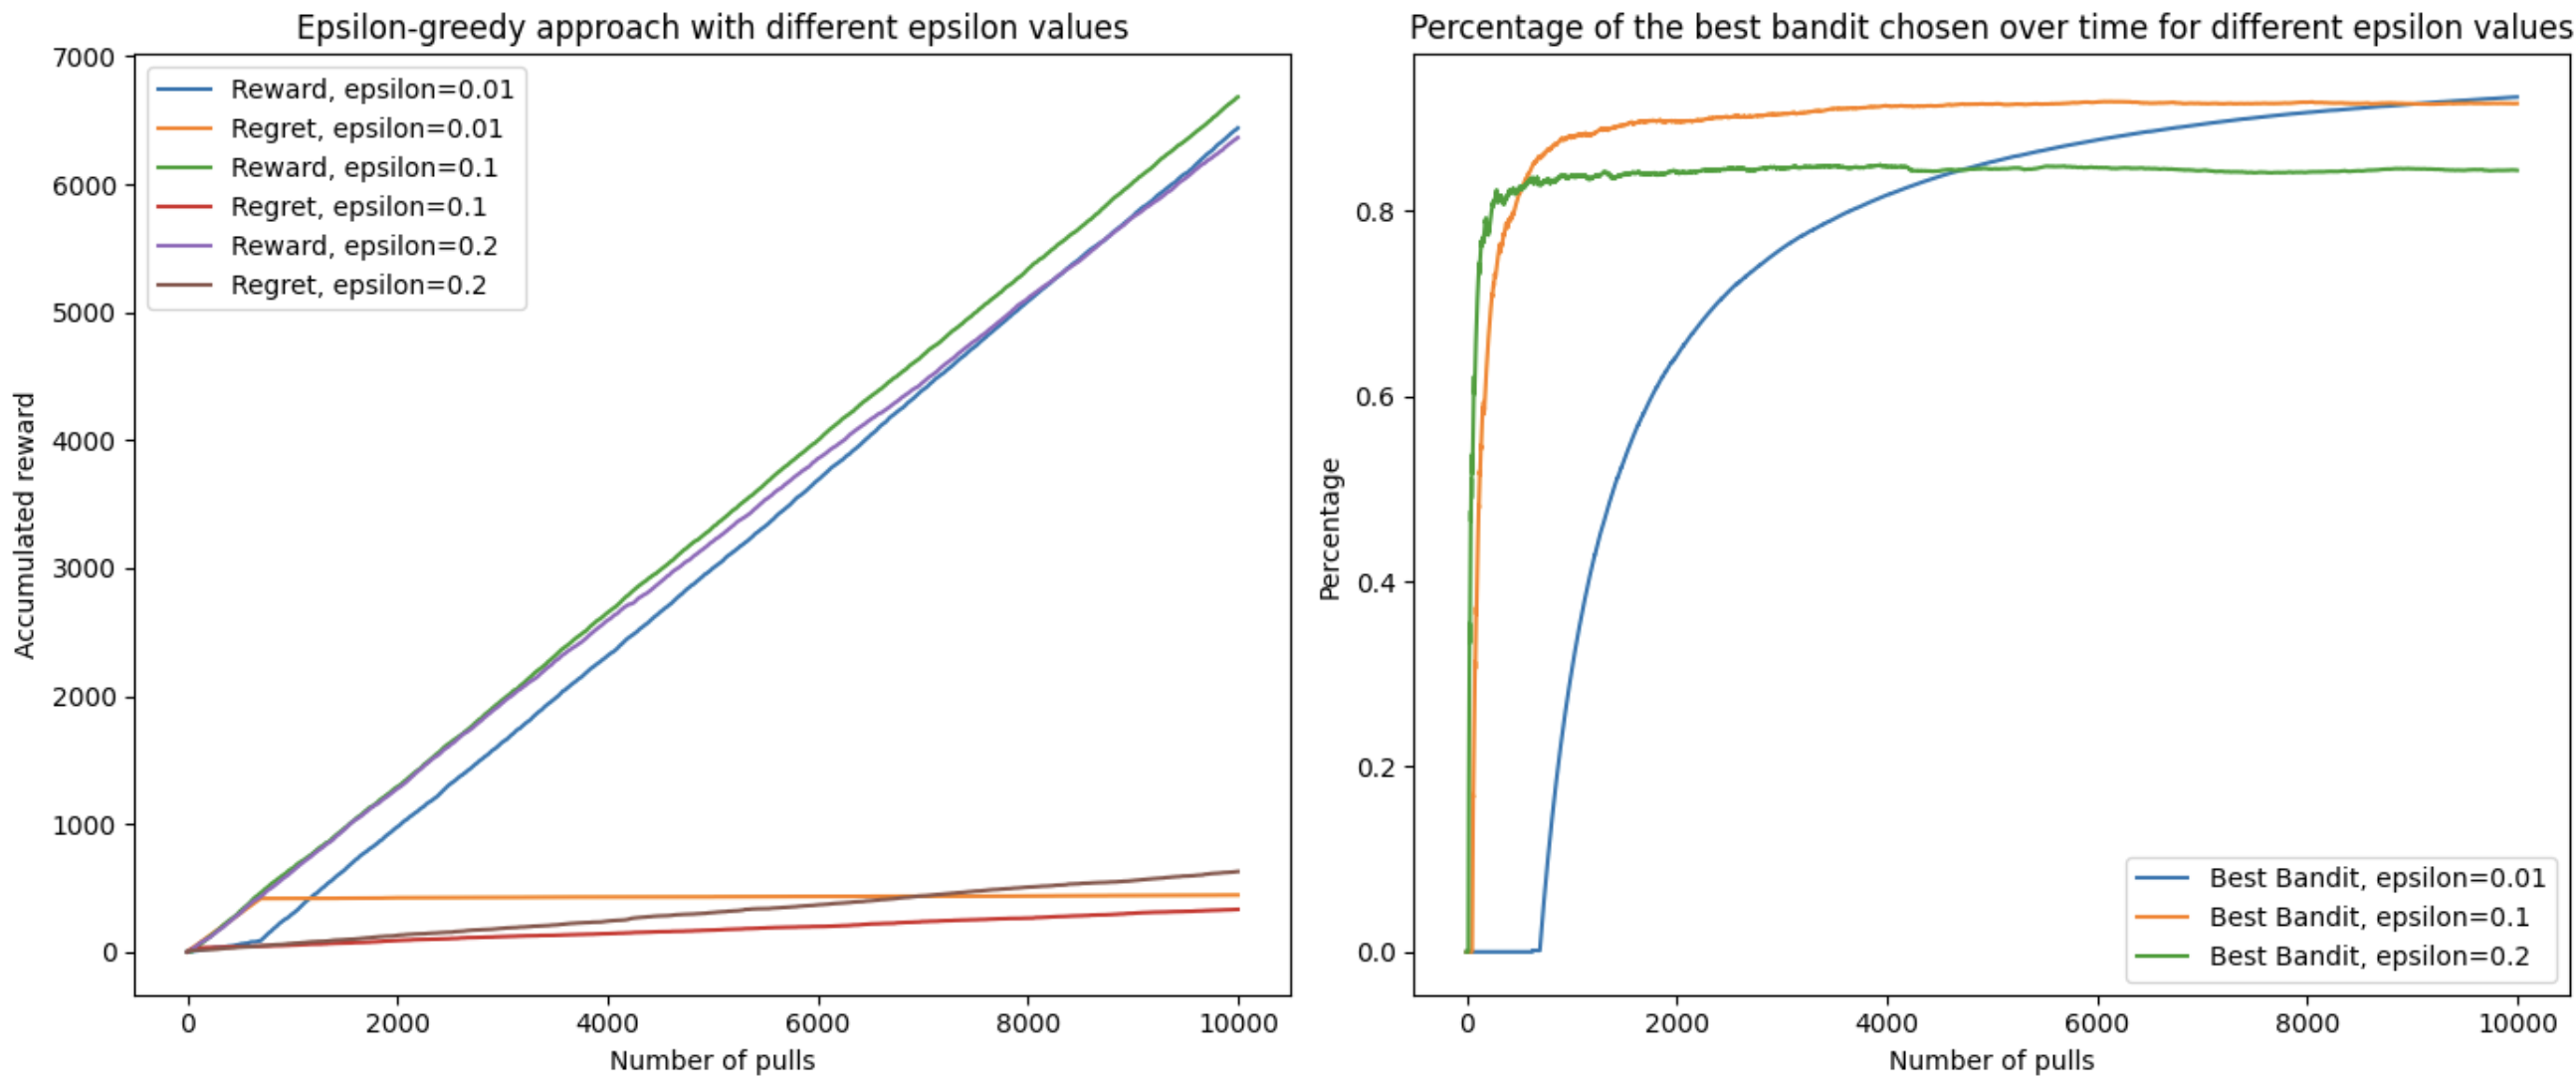
\includegraphics[width=0.9\textwidth]{images/1.1.b}
		\caption{Epsilon-greedy approach with different epsilon values (0.01, 0.1, 0.02) averaged over 100 runs (left) and Percentage of bandits chosen over time for different epsilon values (right)}
		\label{fig:1.1.b}
	\end{figure}
	
	\newpage
	
	\subsection{1.1.c}
	
	Learnings: As we can see, the optimistic initialization is better, as it finds the best bandit much faster in most cases (see \ref{fig:1.1.c.1} right and \ref{fig:1.1.c.2}) leading to more reward and less regret for this init (see \ref{fig:1.1.c.1} left). In some cases though, the optimistic approach can backfire, as a worse bandit is chosen and exploited in the beginning, until the actual best bandit is chosen and exploited.
	
	We tried to average the results but ran into a shape transformation error (array mapping), which we could not resolve for the life of us. 
	\newline
	\begin{figure}[h!]
		\centering
		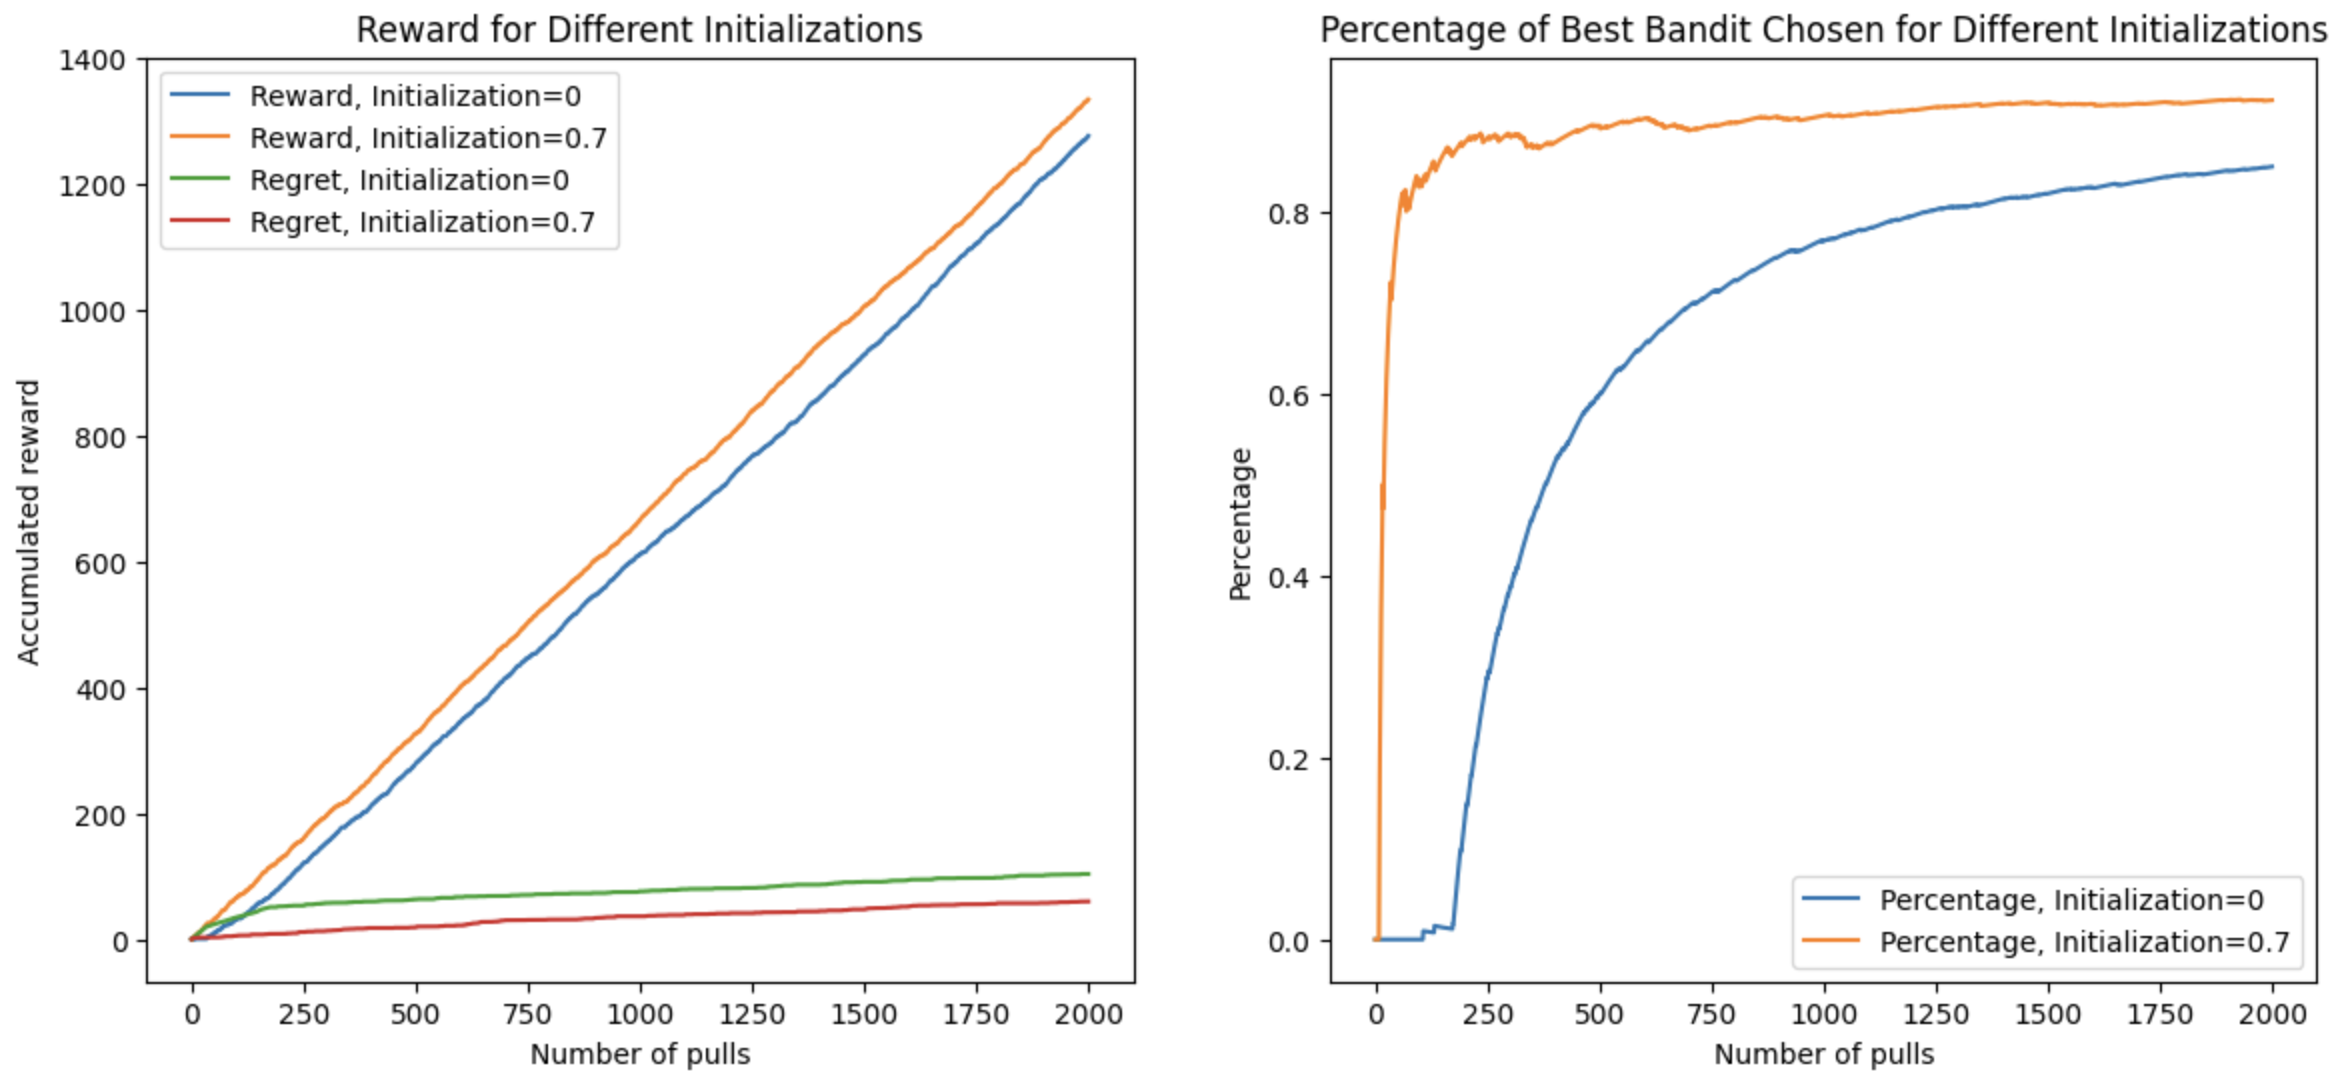
\includegraphics[width=0.9\textwidth]{images/1.1.c.1}
		\caption{Reward for Different Initializations (left) and Percentage for Best Bandit Chosen for Different Intializations}
		\label{fig:1.1.c.1}
	\end{figure}
	\begin{figure}[h!]
		\centering
		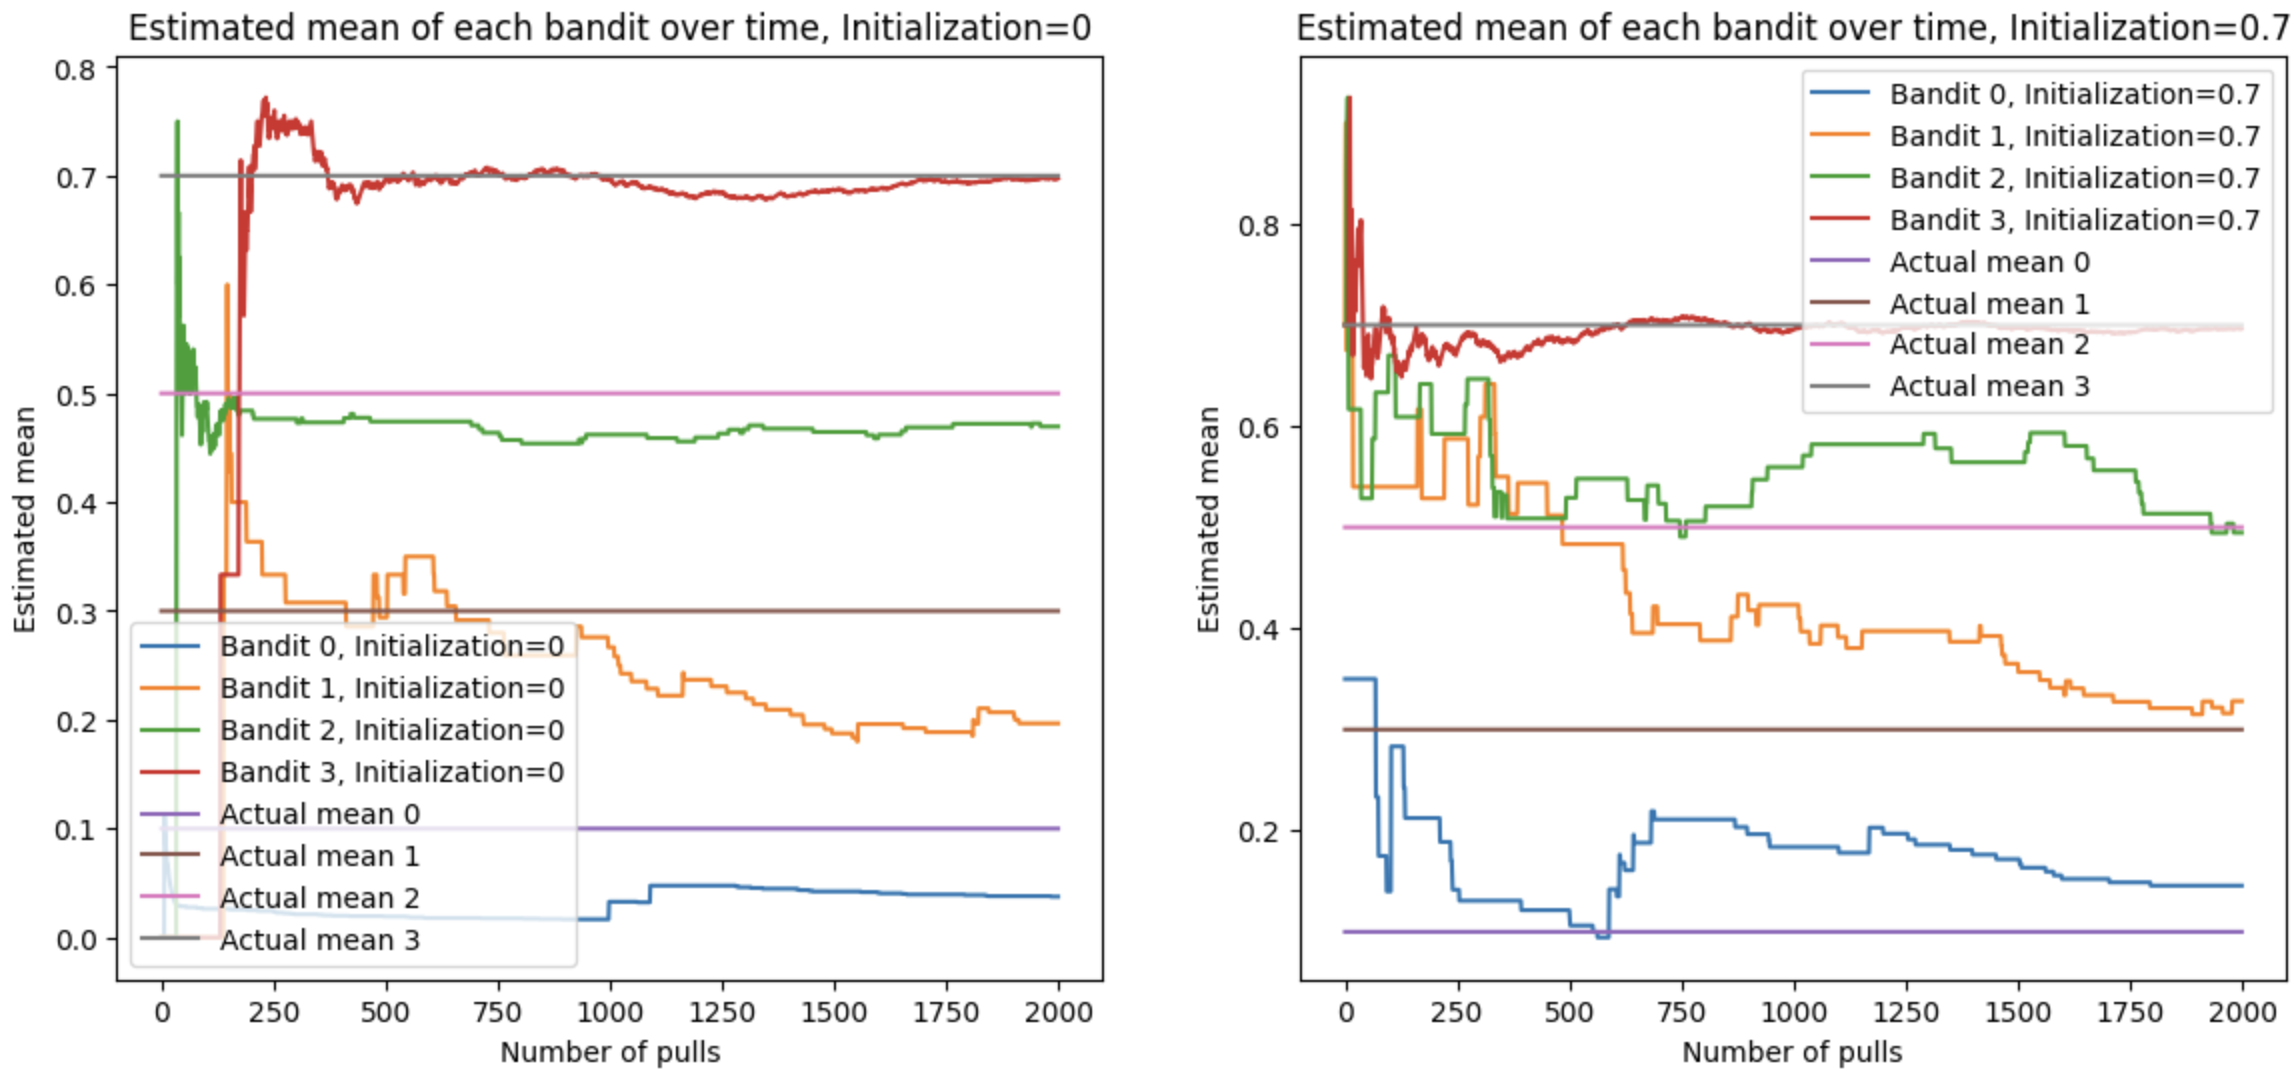
\includegraphics[width=0.9\textwidth]{images/1.1.c.2}
		\caption{Estimated mean of each bandit over time. Initialization = 0 (left) and Initialization = 0,7 (right)}
		\label{fig:1.1.c.2}
		
	\end{figure}
	\newpage
	
	\subsection{1.1.d}
	We defined the epsilons using 100 ones in the and then a 1/x function starting from 1 going to 0.01.
	
	Learnings: If we model the epsilon values in a 1/x fashion, going from 1 down to 0.01, we get a high exploration rate in the beginning, which is necessary to first find the best bandit. After some time, we can be pretty sure we have chosen the right bandit and we can exploit it using smaller epsilon values.
	
	The results show, that the two algorithms start of pretty similar but then start to drift apart regarding Reward and Regret (see \ref{fig:1.1.d} left). This means that the Adaptive epsilon greedy is outperforming the normal epsilon greedy algorithm.
	\newline
	\begin{figure}[h!]
		\centering
		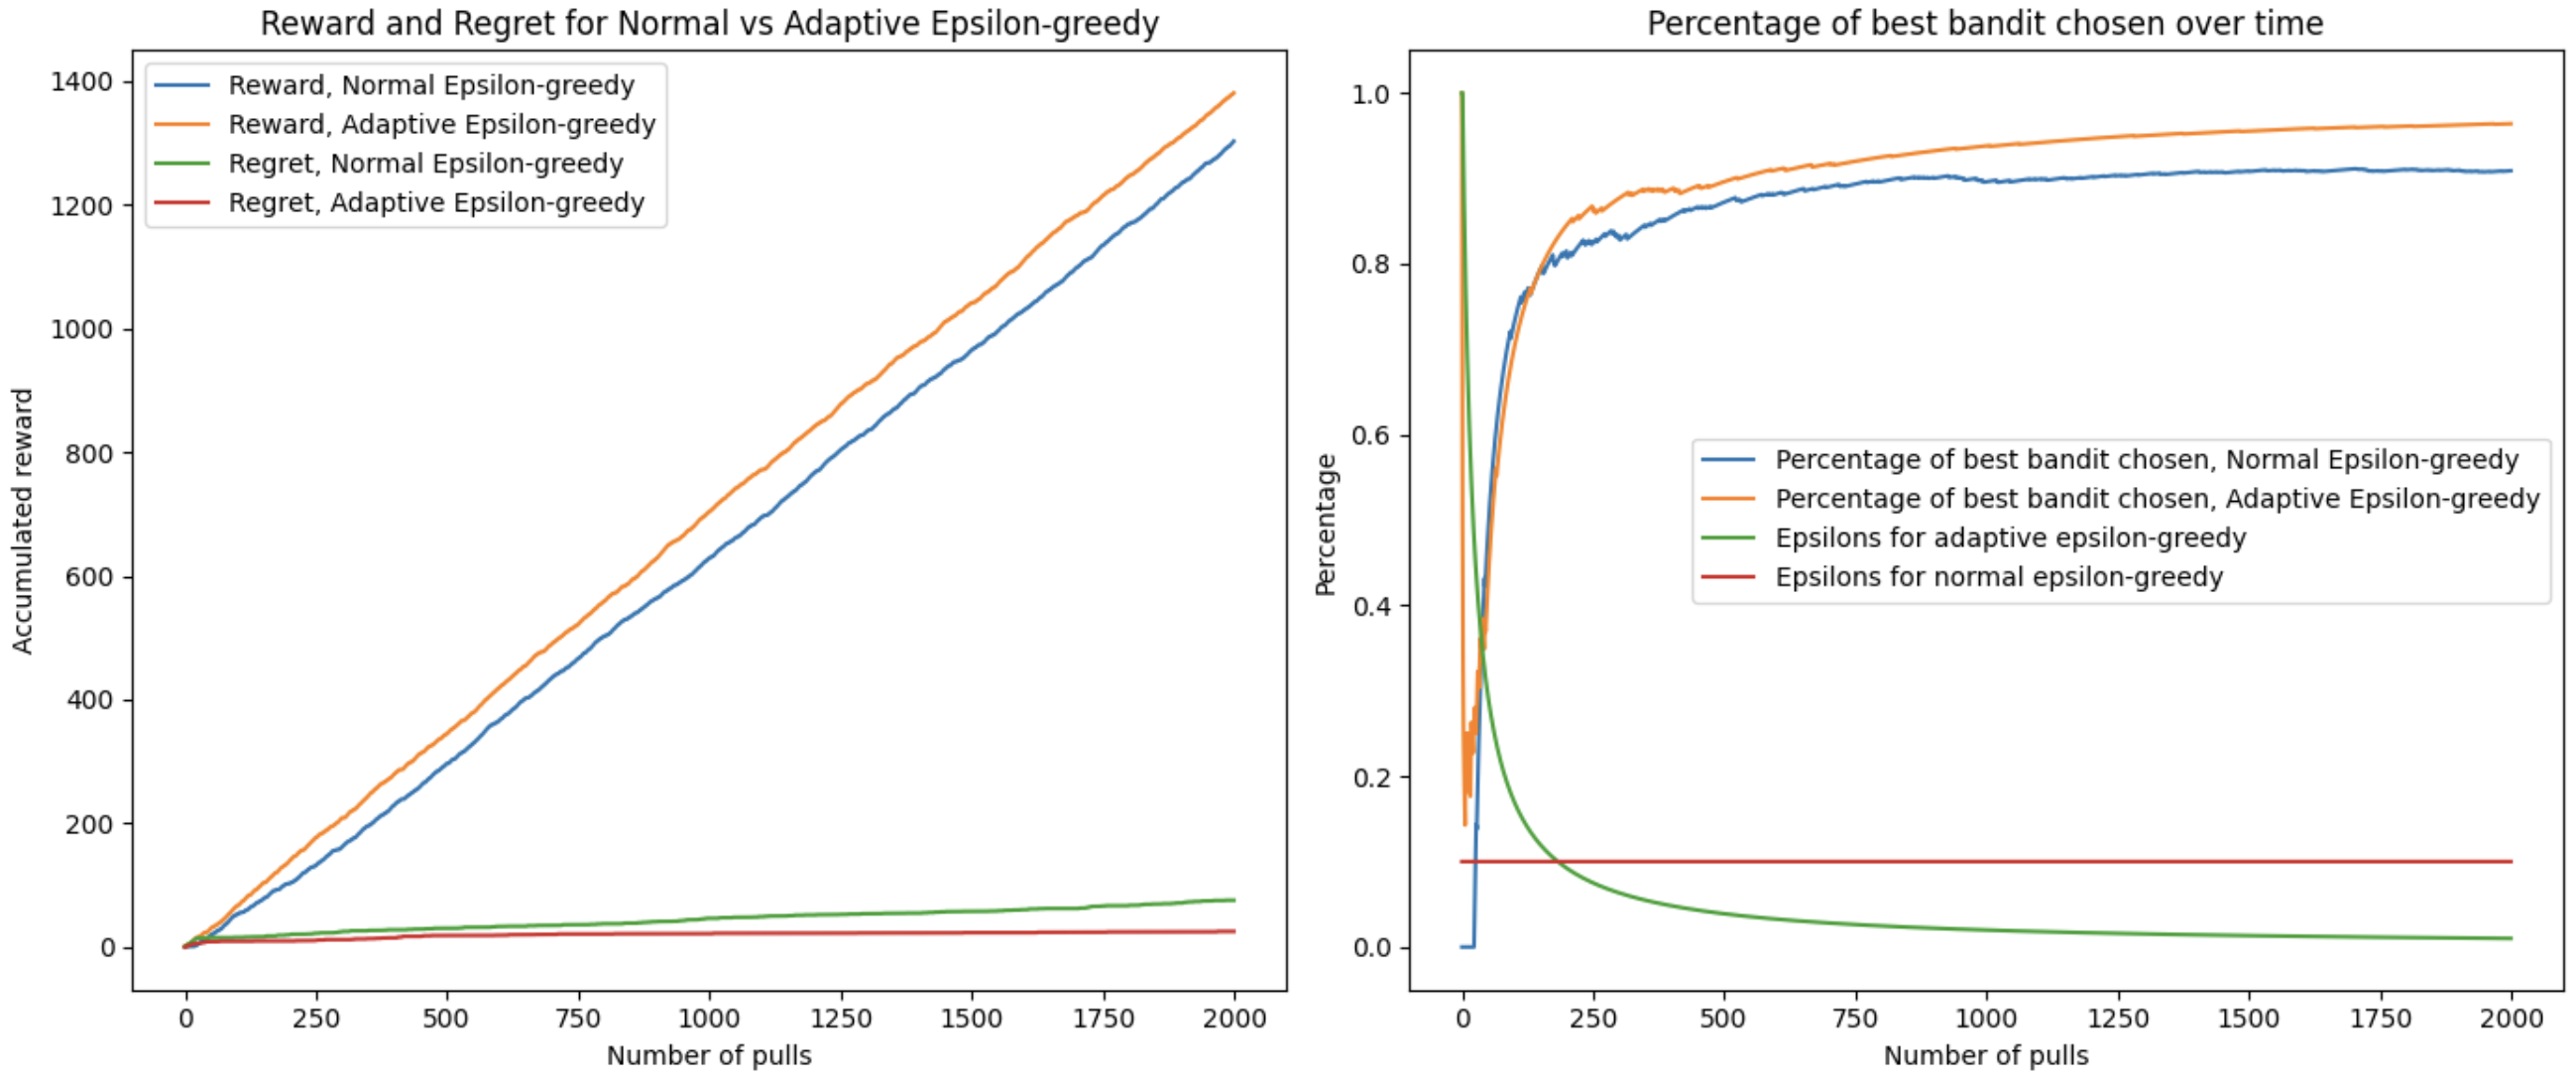
\includegraphics[width=0.9\textwidth]{images/1.1.d}
		\caption{Reward and Regret for Normal vs. Adaptive Epsilon-greedy (left) and Percentage of best bandit chosen over time (right)}
		\label{fig:1.1.d}
		
	\end{figure}
	
	
	\section{Exercise 1.2}
	\subsection{1.2.a}
	The non-stationary Bandit problem means, that the actual rewards of each bandit change over time, meaning that information about the current estimated rewards are less conclusive. A possible algorithmic solution should weigh the results from recent pulls greater than those which lie further in the past. Our approach is an exponentially decreasing weight distribution, assigning a weight of 1 to the most recent pull and a weight close to 0 to the first one. This way, we do not need to assume anything about the change of probability over time, while still not relying on outdated data.
	Exploration needs to be constantly prioritised in this case, since there is never a point at which one bandit can be exploited with certainty. A decreasing epsilon is thus not a valid approach, as it assumes that the accuracy of the reward estimation increases over time.
	The algorithms can be evaluated by calculating the total reward over a great number of pulls, and by analysing how quickly the algorithm adapts to changes in the bandit probability.
	
	\subsection{1.2.b}
	Adjusting the bandit problem to be nonstationary: Let all initial means be the same value, lets say 0.5. We will change the means of the bandits over time by adding random values based on a normal distribution with mean 0 and standard deviation 0.01. 
	
	\subsection{1.2.c}
	
	As we can see, the epsilon-greedy algorithm has a tough time adapting to the changing environment. The estimated means are not able to adapt to the changing actual means of the bandits. Therefore we see a very high regret, which in some runs sometimes even overtakes the reward (see \ref{fig:1.2.c.1} left). We also detect 3 different bandits being use at a high percentage over the course of the run. This is due to the estimated mean of each bandit shifting heavily throughout execution (see figure \ref{fig:1.2.c.2} left)- a direct result from the varying estimated results for each bandit. Another problem poses the difference in estimated mean and actual mean of the bandits. Figure \ref{fig:1.2.c.2} shows this discrepancy very predominantely in bandit 2: It has the highest estimated mean, but places lowest in the actual mean when compared to the other bandits. Furthermore, the bandit 0, which is set to overcome bandit 3 regarding value of the actual mean, is placed lowest in estimated mean. To fix this, the algorithm would have to unexectedly explore the bandits to account for these drastic changes in actual mean. 
	
	\begin{figure}[h!]
		\centering
		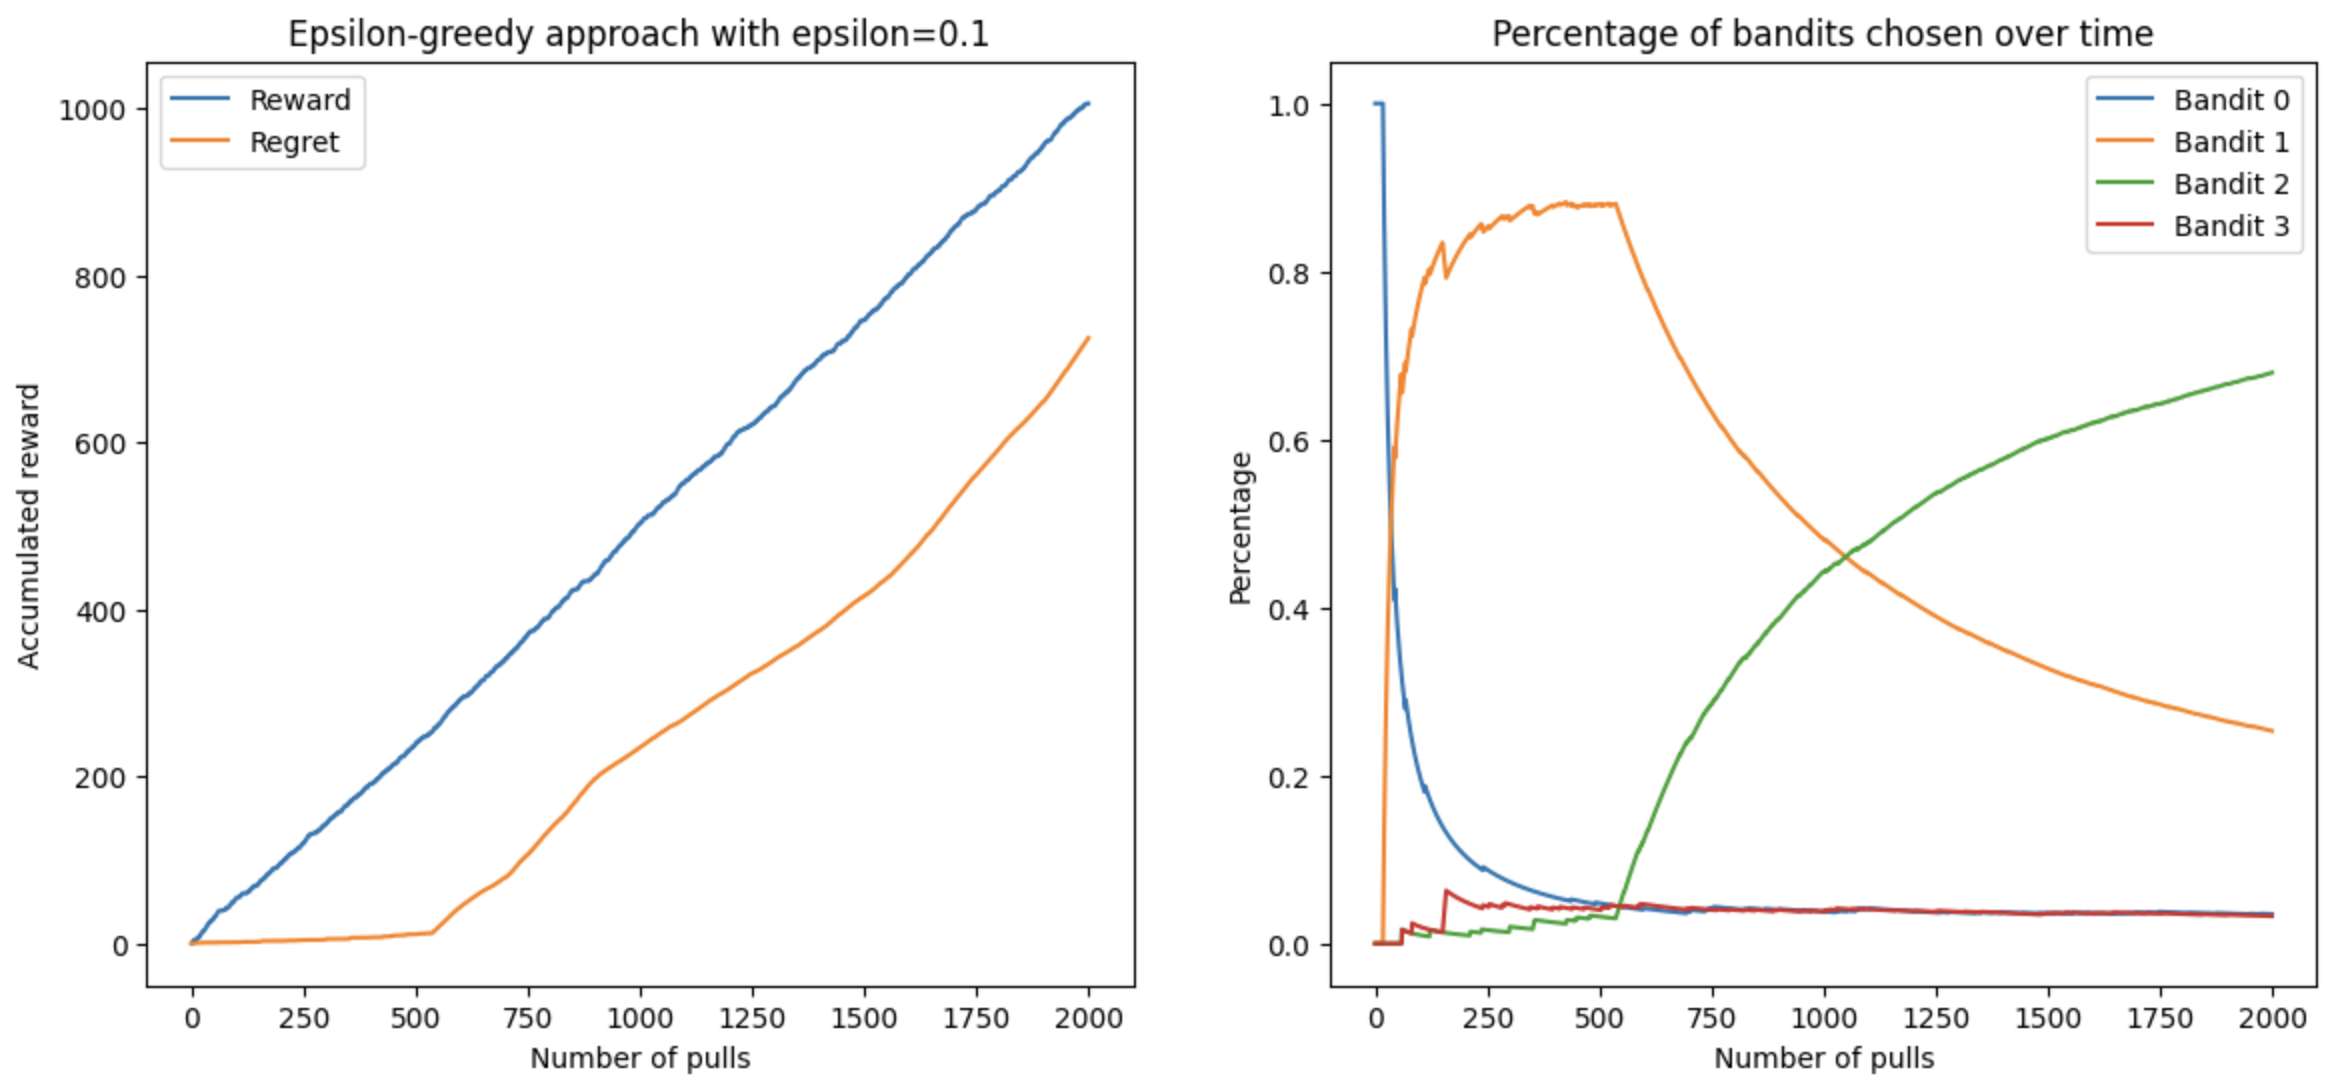
\includegraphics[width=0.8\textwidth]{images/1.2.c.1}
		\caption{Epsilon greedy approach with epsilon = 0.1 for non-stationary bandits (left) and Percentrage of bandits chosen over time (right)}
		\label{fig:1.2.c.1}
		
	\end{figure}
	
	\begin{figure}[h!]
		\centering
		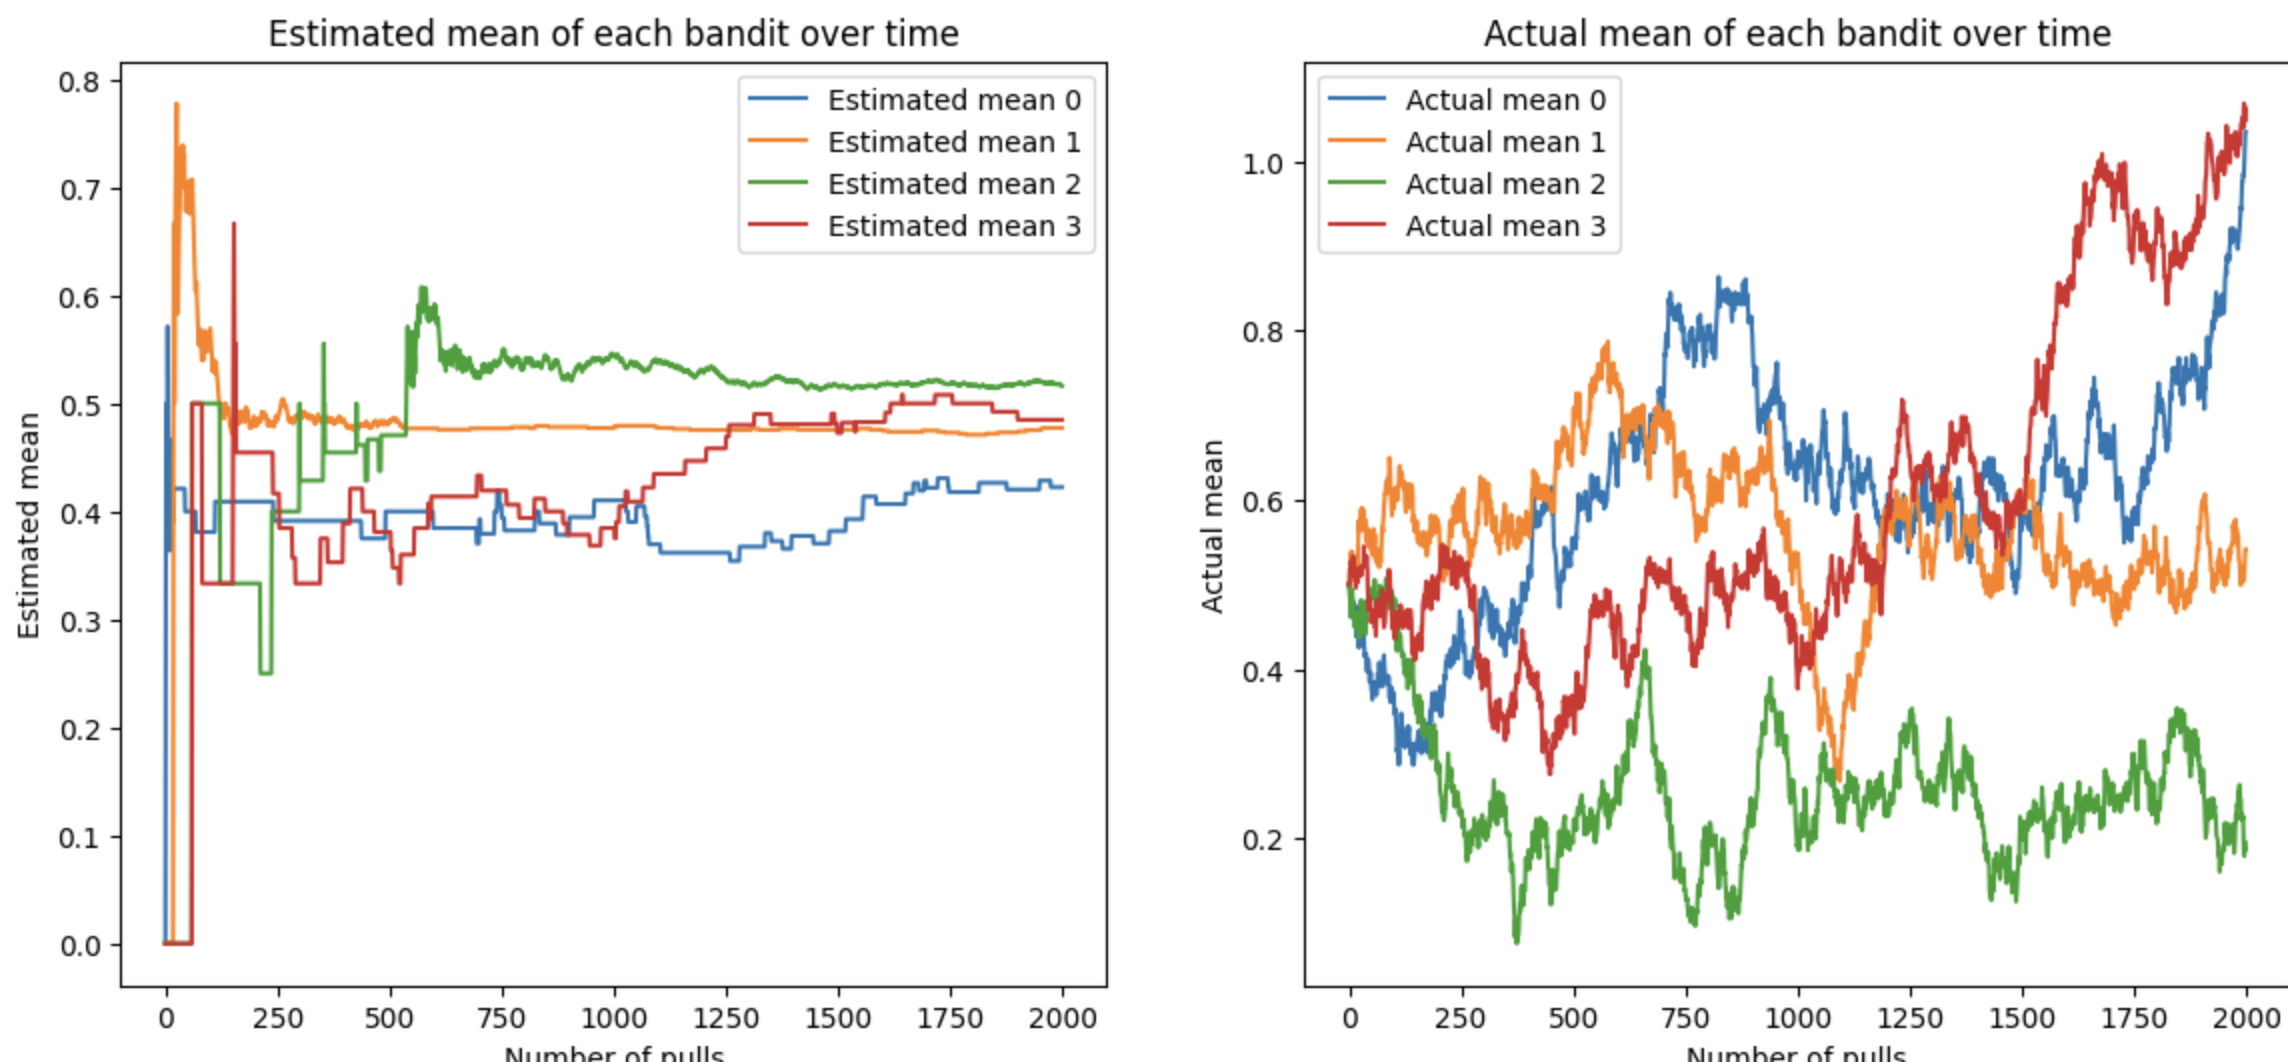
\includegraphics[width=0.8\textwidth]{images/1.2.c.2}
		\caption{Estimated mean of each bandit over time (left) vs. actual mean of each bandit(right)}
		\label{fig:1.2.c.2}
		
	\end{figure}
	
	\newpage
	
	\subsection{1.2.d}
	Possible adjustments to the epsilon-greedy algorithm to improve its performance for the non-stationary bandit problem: 
	
	\begin{itemize}
		\item We could use a dynamic epsilon value over time, such that the algorithm does more exploring in the non-stationary environment. 
	 \item We could give more weight to the more recent data points, since old information might not be as important. 
	\item  We could use a different algorithm that is better suited for non-stationary bandit problems. 
	\item All in all: We should try balancing the exploitation of learned information while not neglecting the exploration in a shifting environment. 
\end{itemize}
\end{document}